\documentclass[a4paper,10pt]{article}
\usepackage[utf8]{inputenc}
\usepackage[margin=1.5cm, bottom=2cm]{geometry}
\usepackage{fancyhdr}
\usepackage{enumitem}
\usepackage{xcolor}
\usepackage[most]{tcolorbox}
\newtcolorbox{osservazioni}{
  colback=gray!8,    % sfondo grigio chiaro
  colframe=white,      % nessun bordo
  arc=2mm,            % angoli smussati
  boxrule=0pt,        % spessore bordo 0
  fontupper=\footnotesize,
  left=2mm, right=2mm, top=2mm, bottom=2mm,
  before skip=7pt,   % niente spazio prima
  after skip=15pt     % niente spazio dopo
}
\pagestyle{fancy}
\usepackage{tikz}
\usetikzlibrary{automata, positioning}
\pagestyle{fancy}


%%%%%%%%%%%%%%%%%%%
\newcommand{\EsercitazioneNum}{04}
\newcommand{\Data}{14/09/2025}
%%%%%%%%%%%%%%%%%%%

% Numero di pagina in basso al centro
\fancyhf{}
\fancyfoot[C] \thepage
\renewcommand{\footrulewidth}{0pt} % niente linea in basso
\renewcommand{\headrulewidth}{0pt} % niente linea in alto

\begin{document}
\footnotesize  % font generale più piccolo

\noindent
\small \textbf{Computabilità, Complessità e Logica - a.a. 2025/26} \hfill \textbf{Esercitazione \EsercitazioneNum} \\[0.2cm]
\scriptsize Matteo Liotta, \texttt{matteo.liotta@studenti.units.it} \hfill \Data \\[0.2cm]

\noindent\makebox[\linewidth]{\rule{\linewidth}{0.4pt}} \\[1cm]


\noindent\Large \textbf{Esercitazione \EsercitazioneNum}: \textit{Espressioni regolari e linguaggi regolari}
\begin{osservazioni}
    \textbf{\textit{Nota}}. Sono indicati in \textcolor{blue}{\textit{blu}} gli esercizi che non saranno trattati durante l'esercitazione, bensì lasciati come strumento aggiuntivo di esercitazione individuale. Resta comunque assoluta disponibilità per la loro risoluzione negli incontri successivi, qualora necessario.
\end{osservazioni}

{\normalsize
\begin{itemize}[label=, leftmargin=0pt]


\item\underline{\textit{\textbf{Scrittura dell'espressione regolare equivalente ad un automa regolare}}}

    \item \textbf{Esercizio 1. (**)}\\ Si consideri il seguente automa regolare definito su $\Sigma =\{a,b\}$. Si individui l'espressione regolare corrispondente, indicando chiaramente i passi intermedi.
    {
    \small
    \begin{center}
	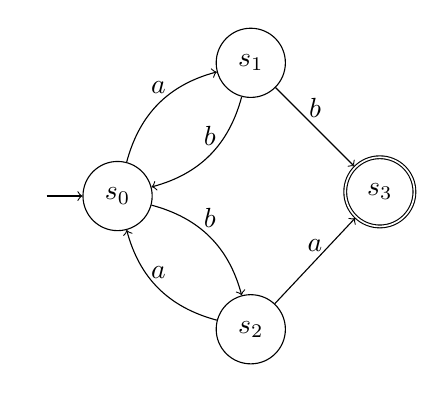
\begin{tikzpicture}
		\node[state, initial, initial text=] (A) {$s_0$};
		\node[state] (B) [above right=1.5of A] {$s_1$};
		\node[state] (C) [below right=1.5of A] {$s_2$};
		\node[state, accepting] (D) [below right=of B] {$s_3$};
		
		\path[->] 
        (A) edge[above, bend left] node{$a$} (B)
		(B) edge[above] node{$b$} (D)
		(A) edge[above, bend left] node{$b$} (C)
		(C) edge[above] node{$a$} (D)
		(B) edge[above, bend left] node{$b$} (A)
		(C) edge[above, bend left] node{$a$} (A);
    \end{tikzpicture}
    \end{center}
    }

    \item \textbf{\textcolor{blue}{Esercizio 2. (**)}}\\ Si consideri il seguente automa regolare definito su $\Sigma =\{a,b\}$. Si individui l'espressione regolare corrispondente, indicando chiaramente i passi intermedi.

    {
    \small
    \begin{center}
	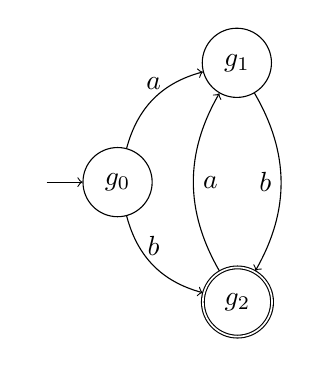
\begin{tikzpicture}
    	\node[state, initial, initial text=] (A) {$g_0$};
    	\node[state] (B) [above right=1.25of A] {$g_1$};
    	\node[state, accepting] (C) [below right=1.25of A] {$g_2$};
    %	\node[state, accepting] (D1) [right=of B] {$g_3$};
    %	\node[state, accepting] (D2) [right=of C] {$g_4$};
    %		
    	\path[->] (A) edge[above, bend left] node{$a$} (B)
    	 (B) edge[left, bend left] node{$b$} (C)
      (A) edge[above, bend right] node{$b$} (C)
      (C) edge[right, bend left] node{$a$} (B);
    %	\draw (D1) edge[above, bend left] node{$a$} (B);
    %	\draw (D2) edge[above, bend left] node{$b$} (C);
    
    \end{tikzpicture}
    \end{center}
    }
  



    \item \textbf{Esercizio 3. (**)}\\ Si consideri il seguente automa regolare definito su $\Sigma =\{a,b\}$. Si individui l'espressione regolare corrispondente, indicando chiaramente i passi intermedi.

    {
    \small

\begin{center}
	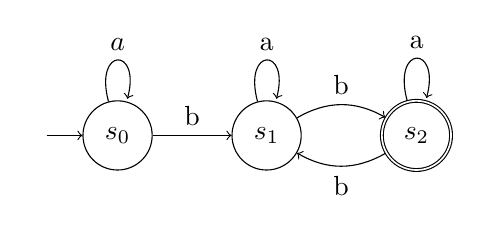
\begin{tikzpicture}
        \node[state, initial, initial text=] (A) {$s_0$};
        \node[state, right= of A] (B) {$s_1$};
        \node[state, accepting, right= of B] (C) {$s_2$};
%	
		\path[->] 
        (A) edge [loop above] node{$a$} (A)
            edge [above] node{b} (B)
        (B) edge [loop above] node{a} (B)
            edge [bend left, above] node{b} (C)
        (C) edge [bend left, below] node{b} (B)
            edge [loop above] node{a} (C);
            
        
	\end{tikzpicture}
\end{center}
    }

        \item \textbf{\textcolor{blue}{Esercizio 4. (*)}}\\ Si consideri il seguente automa regolare definito su $\Sigma =\{a,b\}$. Si individui l'espressione regolare corrispondente, indicando chiaramente i passi intermedi.
    {
    \small
    \begin{center}
    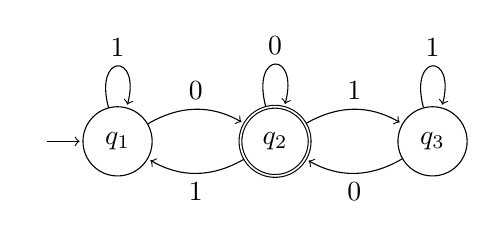
\begin{tikzpicture}[shorten >=1pt, node distance=2cm, on grid, auto]
        \node[state, initial, initial text=] (q1)   {$q_1$};
        \node[state, accepting] (q2) [right=of q1] {$q_2$};
        \node[state] (q3) [right=of q2] {$q_3$};
        
        \path[->]
        (q1) edge [bend left] node {0} (q2)
             edge [loop above] node {1} ()
        (q2) edge [loop above] node {0} ()
             edge [bend left] node {1} (q3)
             edge [bend left] node {1} (q1)
        (q3) edge [loop above] node {1} ()
             edge [bend left] node {0} (q2);
         
    \end{tikzpicture}
    \end{center}
    }

    \vfill
    \noindent\makebox[\linewidth]{\rule{\linewidth}{0.4pt}}
    \newpage
    {\noindent
    \small \textbf{Computabilità, Complessità e Logica - a.a. 2025/26} \hfill \textbf{Esercitazione \EsercitazioneNum} \\[0.2cm]
    \scriptsize Matteo Liotta, \texttt{matteo.liotta@studenti.units.it} \hfill \Data \\[0.2cm]
    \noindent\makebox[\linewidth]{\rule{\linewidth}{0.4pt}} \\[0.3cm]}


\underline{\textit{\textbf{Identificazione del linguaggio regolare definito da una espressione regolare}}}
    
    \item \textbf{Esercizio 5. (**)}\\ Si consideri la seguente espressione regolare su $\Sigma=\{a,b,\#\}$
    {\begin{center}
        $\bigg((T\cdot R)^* \cdot \#\bigg)^*$
    \end{center}} 
    dove:
    \begin{itemize}[label=]
        \item $T=\{b^k:\leq 4\}$
        \item $R =\{a^2, a^4, a^6\}$
    \end{itemize}
    Si indichi il linguaggio definito dall'espressione regolare in questione.\\

    \item \textbf{Esercizio 6. (**)}\\ Si consideri la seguente espressione regolare su $\Sigma=\{a,b,\#\}$
    {\begin{center}
        $\bigg( \quad \bigg((a+b)^*\cdot(bc+dc^*)\bigg) \cdot b\quad\bigg)^*$
    \end{center}} 
    Si costruisca l'automa regolare tale da riconoscere il linguaggio definito dall'espressione regolare proposta.\\

    \item \textbf{\textcolor{blue}{Esercizio 7. (**)}}\\ Si consideri la seguente espressione regolare su $\Sigma=\{a,b,\#\}$
    {\begin{center}
        $\bigg(\quad \bigg((a + b)\cdot (b +c)\bigg)^*\cdot (c + d)^*\quad \bigg)^*$
    \end{center}} 

    
    Si costruisca l'automa regolare tale da riconoscere il linguaggio definito dall'espressione regolare proposta.\\


    
\end{itemize}
}
\vfill
\noindent\makebox[\linewidth]{\rule{\linewidth}{0.1pt}}
\end{document}
